\documentclass{article}
\usepackage{fullpage,palatino,mathpazo,amsmath,amssymb,url}
\usepackage{url,amsmath,amssymb,subfigure,boxedminipage,shadow}
\usepackage[pdftex]{graphicx,color}
%\usepackage{hevea}
\graphicspath{{Figures/}}

\newcommand{\operator}{ \verb!Operator! }

\title{\scalebox{0.3}{\mbox{\input{../Figures/flopocoLogo.pdf_t}}}\\
FloPoCo \input{../../VERSION} developer manual
}

\author{Florent de Dinechin, Bogdan Pasca}

\graphicspath{{../Figures/}}
\pagestyle{empty}

\begin{document} 
\sloppy



\maketitle


Welcome to new developers! 

The purpose of this document is to help you use FloPoCo in your own
project (section~\ref{sec:linking}), and to show you how to design your own pipelined operator
using the FloPoCo framework (section~\ref{sec:pipeline-made-easy}). 

 \section{Getting started with FloPoCo\label{sec:getting-started}}


\subsection{Getting the source and compiling using CMake}

It is strongly advised that you work with the svn version of the
source, which can be obtained by following the instructions on
\url{https://gforge.inria.fr/scm/?group_id=1030}. If you wish to
distribute your work with FloPoCo,  contact us.

If you are unfamiliar with the CMake system, there is little to learn,
really. When adding .hpp and .cpp files to the project, you will need
to edit \texttt{CMakeLists.txt}. It is probably going to be straightforward,
just do some imitation of what is already there. Anyway \texttt{cmake} is well
documented. The web page of the CMake project is \url{http://www.cmake.org/}.


\subsection{Overview of FloPoCo}

In FloPoCo, everything is an \texttt{Operator}. Operator is a virtual
class, all FloPoCo operators inherit this class. A good way to design
a new operator is to imitate a simple one. We suggest
%\texttt{IntAdder} or 
\texttt{Shifter} for simple integer operators, and \texttt{FPAdderSinglePath}
for a complex operator with several sub-components. An example of
assembling several FP operators in a larger pipeline is
\texttt{Collision}.

 Meanwhile, browse
through \texttt{Operator.hpp}. It has become quite bloated, showing
the history of the project. Try not to use methods flagged as
deprecated, as they will be removed in the future.  Instead, use the
automatic pipeline framework is described in Section~\ref{sec:pme}
below.

Another important class hierarchy in FloPoCo is \texttt{Target}, which
defines the architecture of the target FPGA. It currently has several sub-classes 
including, \texttt{VirtexIV, 5, 6} and \texttt{StratixII, IV}. You may want to
add a new target, the best way to do so is by imitation. Please
consider contributing it to the project.

To understand the command line, go read \texttt{main.cpp}. It is not
the part we are the most proud of, but it does the job.

The rest is arithmetic!

And do not hesitate to contact us: \texttt{Florent.de.Dinechin} or
\texttt{Bogdan.Pasca}, at \texttt{ens-lyon.fr}

\begin{center}
%  \begin{latexonly}
  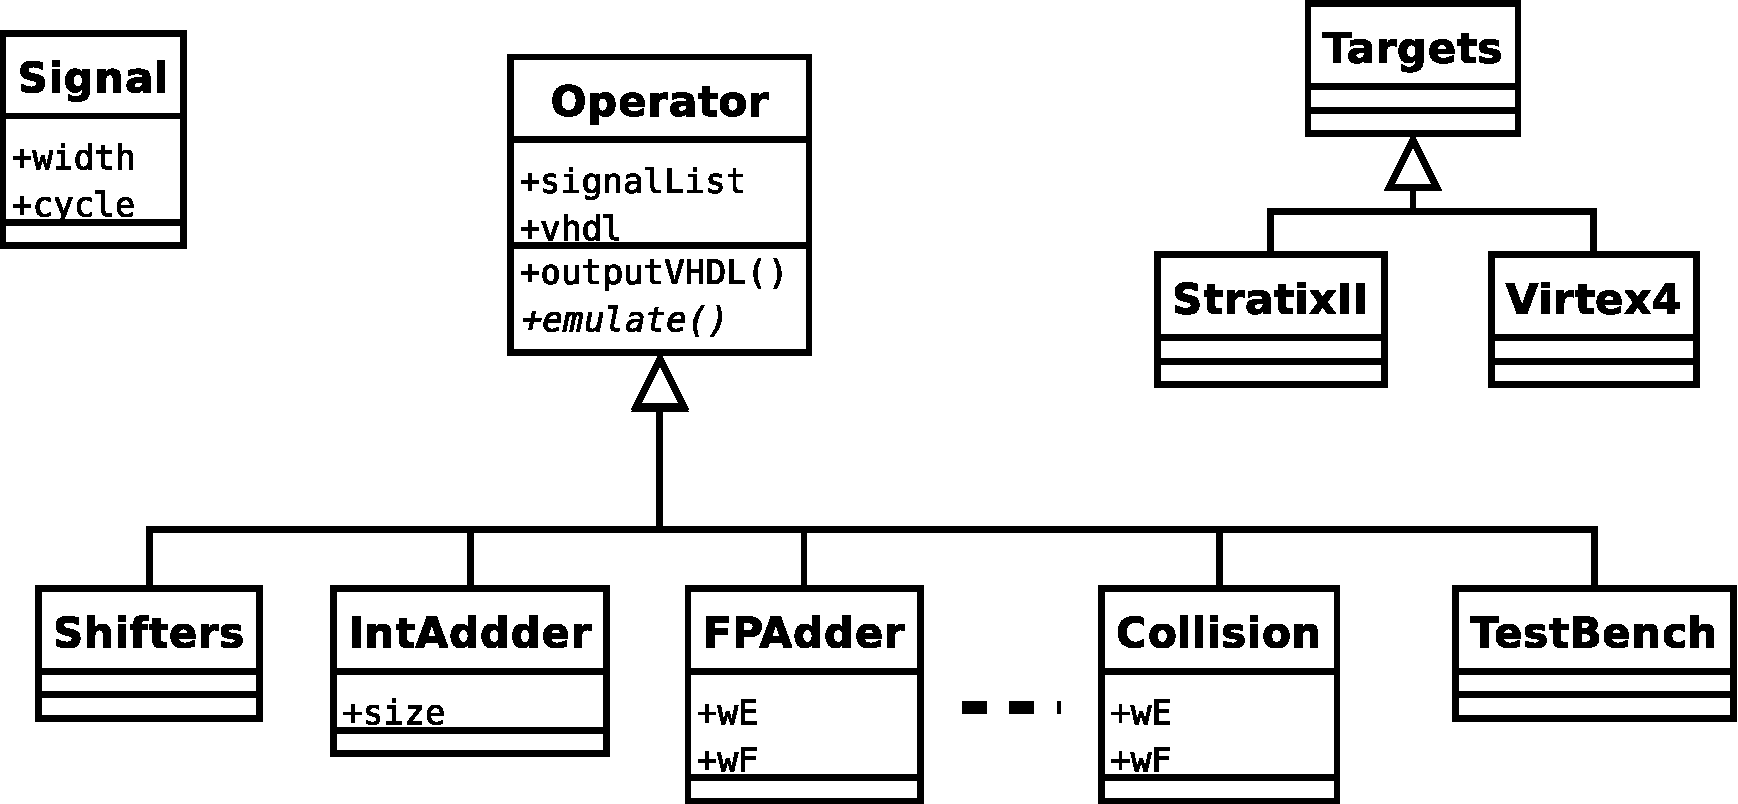
\includegraphics[width=0.7\textwidth]{../Figures/FloPoCoClasses.pdf}        
%  \end{latexonly}
\end{center}

\section{Linking against FloPoCo\label{sec:linking}}
All the operators provided by the FloPoCo command line are availaible
programmatically in libFloPoCo. A minimal example of using this
library is provided in \texttt{src/main\_minimal.cpp}.

The file \texttt{src/main.cpp} is the source of the FloPoCo command
line, and as such uses most operators: looking at it is the quickest
way to look for the interface of a given operator.

The other way is, of course, to look at the corresponding \texttt{hpp}
file -- they are all included by \texttt{src/Operator.hpp}. Some
operators offer more constructors (richer interface options) than what
is used in \texttt{src/main.cpp}.

There should be a Doxygen documentation of FloPoCo.

\section{Pipelining made easy: a tutorial \label{sec:pipeline-made-easy}}
\label{sec:pme}


If you want to experiment with a dummy operator and try the notions
used in this section, consider reading and modifying the file
\texttt{UserDefinedOperator.hpp} and \texttt{.cpp}. They contain an
operator class \texttt{UserDefinedOperator} that you may freely modify
without disturbing the rest of FloPoCo.


Let us consider a toy MAC unit, which in VHDL would be written
\begin{verbatim}
library ieee;
use ieee.std_logic_1164.all;
use ieee.std_logic_arith.all;
use ieee.std_logic_unsigned.all;
library work;

entity MAC is
   port ( X   : in  std_logic_vector(63 downto 0);
          Y,Z : in  std_logic_vector(31 downto 0);
          R : out  std_logic_vector(63 downto 0)   );
end entity;

architecture arch of MAC is
  signal T: std_logic_vector(63 downto 0);
begin
   T <= Y * Z;
   R <= X + T;
end architecture;
\end{verbatim}

We chose for simplicity a fixed-size operator, but all the following
works as well for parameterized operators.

We have above the description of a combinatorial circuit. We now show how to
turn it into a pipelined one.


\subsection{First steps in FloPoCo operator writing}

FloPoCo mostly requires you to copy the part of the VHDL that is
between the \texttt{begin} and the \texttt{end} of the architecture
into the constructor of a class that inherits from
\verb!Operator!. The following is minimal FloPoCo code for
\verb!MAC.cpp!:
\begin{verbatim}
#include "Operator.hpp"

class MAC : public Operator
{
public:
// The constructor
MAC(Target* target): Operator(target)
{
	setName("MAC");
	setCopyrightString("ACME MAC Co, 2009");		

	// Set up the IO signals
	addInput ("X"  , 64);
	addInput ("Y"  , 32);
	addInput ("Z"  , 32);
	addOutput("R"  , 64);

   vhdl << declare("T", 64) << " <= Y * Z;" << endl;
   vhdl << "R <= X + T;" << endl;
}

// the destructor
	~MAC() {}
\end{verbatim}
 
And that's it. \verb!MAC! inherits from \verb!Operator! the method
\verb!outputVHDL()! that will assemble the information defined in the
constructor into synthesizable VHDL. Note that \verb!R! is declared by \verb!addOutput!.

So far we have gained little, except that is is more convenient to
have the declaration of \verb!T! where its value is defined. Let us
now turn this design into a pipelined one.


\subsection{Basic pipeline}

Let us first insert a synchronization barrier between the result of the
multiplication and the adder input. The code becomes: 

\begin{verbatim}
(...)
   vhdl << declare("T", 64) << " <= Y * Z;" << endl;
   nextCycle();
   vhdl << "R <= X + T ;" << endl;
(...)
\end{verbatim}

With the command-line option \verb!-pipeline=yes!, this code will
insert a synchronisation barrier before the adder, delaying \texttt{X}
so that the operator is properly synchronized. It will produce a
combinatorial operator (the same as previously) with
\verb!-pipeline=no!.

How does it work? 
\begin{itemize}\item 
  \verb!Operator! has a \verb!currentCycle! attribute, initially equal to
  zero. The main function of 	\verb!nextCycle()! is to increment \verb!currentCycle!.

\item Every signal declared through \verb!addInput! or \verb!declare!
  has a \verb!cycle! attribute, which represents the cycle at which
  this signal is active. It is 0 for the inputs, and for signals
  declared through \verb!declare()! it is \verb!currentCycle!  at the
  time \verb!declare! was invoked.

\item Every signal also possesses an attribute \verb!lifeSpan! which
  indicates how many cycles it will need to be delayed. This attribute
  is initialized to 0, then possibly increased by each time the signal is used.
  When the \verb!lifeSpan! of a signal \verb!X!  is
  greater than zero, \verb!outputVHDL()! will create \verb!lifeSpan!
  new signals \verb!X_d1!, \verb!X_d2! and so on, and insert registers
  between them. In other words, \verb!X_d2! will hold the value of
  \verb!X! delayed by 2 cycles.

\item FloPoCo scans the VHDL and looks for right-hand side occurrences
  of declared signals. For instance, in the line after the
  \verb!nextCycle!, it finds \verb!X! and \verb!T!. For such signals, it does the following. First,
  it compares \verb!currentCycle! and the
  \verb!cycle! declared for \verb!X!, which we note \verb!X.cycle!.
  \begin{itemize}\item 
    If they are equal, or if \verb!-pipeline=no!, \verb!X! is written to the VHDL untouched.
  \item If \verb!currentCycle! $<$ \verb!X.cycle!, FloPoCo emits an error message complaining that \verb!X! is being
    used before the cycle at which it is defined.
  \item If \verb!currentCycle! $>$ \verb!X.cycle!, FloPoCo delays
    signal \verb!X! by n=\verb!currentCycle!$-$\verb!X.cycle!
    cycles. Technically, it just replaces, in the output VHDL,
    \verb!X! with \verb!X_dn!. It also updates \verb!X.lifeSpan! to be
    at least equal to n.
  \end{itemize}
\item All the needed signals will be declared in the output VHDL based
  on the \verb!lifeSpan! information.
\end{itemize}

This whole scheme is actually run in two passes so that
\verb!currentCycle! may be moved forth and back in the FloPoCo code, which is useful in some situations.

This scheme gracefully degrades to a
combinatorial operator. It also automatically adapts to random
insertions and suppressions of synchronization barriers. Typically,
one synthesizes an operator, and decides to break the critical path by
inserting a synchronisation barrier in it. This may be as simple as
inserting a single \verb!nextCycle()! in the code. FloPoCo takes care of the rest.

It is also possible to have \verb!if!s before some of the
\verb!nextCycle()!, so that the pipeline adapts to the frequency, the
operator generic parameters, etc. See \verb!IntAdder! for an example.
However, starting with version 2.1.0 a finer-grain procedure for pipelining 
operators is introduced and will be explained section \ref{sec:finegrain}.

Some more notes:
\begin{itemize}
\item The second parameter of \verb!declare()!, the signal width, is
  optional and defaults to 1 (a \verb!std_logic! signal).

\item Other functions allow to manipulate \verb!currentCycle!
  \begin{itemize}
  \item 
    \verb!setCycle(int n)! sets \verb!currentCycle! to  $n$.  
  \item \verb!setCycleFromSignal(string s)!  
    sets the \verb!currentCycle! to the \verb!cycle! of the signal
    whose name is given as an argument (going back if needed),
  \item 
    \verb!syncCycleFromSignal(string s)! is similar to the previous but may only advance
    \verb!currentCycle!. It allows to synchronise several
    signals by setting \verb!currentCycle! to the max of their
    \verb!cycle!.

See \verb!FPAdderSinglePath! or \verb!FPLog! for examples of
  such synchronisations. 
  \end{itemize}

All these functions have an optional boolean
  second argument which, if true, inserts in the generated VHDL a
  comment ``-- entering cycle n''.


\item If our toy example, is part of a larger circuit such that X is
  itself delayed, the pipeline will adapt to that.

\end{itemize}


\subsection{Pipeline with sub-components}

We now show how to replace the + and * with FloPoCo pipelined
operators. These operators support frequency-directed pipelining,
which means that the resulting MAC will also have its pipeline depth
automatically computed from the user-supplied frequency (the
\texttt{-frequency} option of the command-line).

\begin{verbatim}
(...)
	// vhdl << declare("T", 64) << " <= Y * Z;" << endl;
	IntMultiplier *my_mult = new IntMultiplier(target, 32, 32);
	oplist.push_back(my_mult); // some day this will be an addOperator method
	inPortMap   (my_mult, "X", "Y"); // formal, actual
	inPortMap   (my_mult, "Y", "Z");
	outPortMap  (my_mult, "R","T");
	vhdl << instance(my_mult, "my_mult"); // 2nd param is the VHDL instance name

	// advance to the cycle of the result
	syncCycleFromSignal("T"); 
	// pipelined operators do not have a register on the output 
	nextCycle();

	// vhdl << "R <= X + T;" << endl;
	IntAdder *my_adder = new IntAdder(target, 64);
	oplist.push_back(my_adder);
	inPortMap   (my_adder, "X", "X");
	inPortMap   (my_adder, "Y", "T");
	inPortMapCst(my_adder, "Cin", "0"); -- carry in
	outPortMap  (my_adder, "R","RR");
	vhdl << instance(my_adder, "my_add");

	// advance to the cycle of the result
	syncCycleFromSignal("RR"); 
   vhdl << "R <= RR;" << endl; 
(...)
\end{verbatim}


And that's it. In the code above, an \verb!inPortMap()! does the same
job as an occurrence of signal on the right-hand side, and an
\verb!outPortMap()! does the same job as a \verb!declare()!, although
it doesn't need a signal width since it can read it from the
sub-component. \verb!instance()! also has the side effect that
\verb!outputVHDL()! will declare this component in the VHDL header of
\verb!MAC!.


\subsection{Frequency-directed pipelining}
\label{sec:finegrain}

The command line of FloPoCo supports specifying the desired frequency
of the generated operators by using the \verb!-frequency! option. The
philosophy behind is to generate the smallest (in terms of resource
usage) and the shorter latency operator given this frequency
specification (\texttt{-frequency} command-line option) for a given
target (\texttt{-target} command-line option).

A fixed pipeline can be easily obtained using the
\verb!nextCycle()! function previously introduced. As suggested before, frequency
directed pipelining can be accomplished by  conditional statements around the 
\verb!nextCycle()!. The following methodology does 
exactly that, but in a generic and (hopefully) future-proof way. 

Let's go back to our basic MAC example (the one without
components). Looking at the critical path it is clear that it goes
through a multiplication and then an addition. Before emitting the
code of an operation that will increase the critical path (in our
example, the multiplication) we want to evaluate in advance what the
critical path becomes if we add to it the delay of this
operation. There are two cases:
\begin{itemize}
\item the new delay is greater than $1/f$. This means that it will be
  impossible to perform these two operations in the same cycle while
  ensuring proper operation at frequency $f$. In this case a
  \verb!nextCycle()!  must be called to insert a
  synchronisation barrier. This resets the critical path delay, which becomes  the
  delay of the operation after the barrier (the multiplication in this
  example).
\item this new critical path delay is smaller than the target period
  ($1/f$). In this case we just have to perform some bookkeeping: the
  critical path delay is incremented with the operation delay.
\end{itemize}

The FloPoCo command that does it all is
\verb!manageCriticalPath(double delay)!. It must be placed before each
block of code that generates some hardware on the critical path --
there is some designer expertise here.

The augmented FloPoCo code would look something like:

\begin{verbatim}
   setCriticalPath(0.0);
   manageCriticalPath( target->DSPMultiplierDelay() );
   vhdl << declare("T", 64) << " <= Y * Z;" << endl;
   manageCriticalPath( target->adderDelay(64) );
   vhdl << "R <= X + T ;" << endl;
\end{verbatim}

Note that the delay passed to \texttt{manageCriticalPath()} should be
evaluated, whenever possible, using methods of the \texttt{Target}
class. This ensure that this pipelining work is done once for all the possible targets. 


\subsection{Sub-cycle pipelining (optional)}

A working pipeline using sub-components is typically obtained by
placing synchronization barriers on the inputs and outputs. However,
it is often an overkill: most of the times, the previous approach
leaves the output cycle not fully consumed. Also, sometimes, one wants
to perform only a very simple, low-delay operation on the inputs.


For such cases, operators can optionally :
\begin{itemize}
	\item receive a list of delays on the inputs ( ("X",1.5e-9),("Y",1.2e-9) ) representing
	the combinatorial delays already present on these signals.
	\item report the combinatorial delay on the output signals ("R", 2.0e-9).
\end{itemize}

Using this information, the sub-component constructor can properly
adjust the pipeline for the given frequency.  Here is full example. The input
delays are given in the variable named \verb!inputDelays!. 

\begin{verbatim}
   setCriticalPath( getMaxInputDelays(inputDelays)  );
   manageCriticalPath( target->DSPMultiplierDelay() );
   vhdl << declare("T", 64) << " <= Y * Z;" << endl;
   manageCriticalPath( target->adderDelay(64) );
   vhdl << "R <= X + T ;" << endl;
   outDelayMap["R"] = getCriticalPath(); //returns the current delay on the critical path
\end{verbatim}

In the case of the second, component-based design, the code becomes:

\begin{verbatim}
	setCriticalPath( getMaxInputDelays(inputDelays)  );
	// vhdl << declare("T", 64) << " <= Y * Z;" << endl;
	IntMultiplier *my_mult = new IntMultiplier(target, 32, 32, inDelayMap("X",getCriticalPath()));
	oplist.push_back(my_mult); // some day this will be an addOperator method
	inPortMap   (my_mult, "X", "Y"); // formal, actual
	inPortMap   (my_mult, "Y", "Z");
	outPortMap  (my_mult, "R","T");
	vhdl << instance(my_mult, "my_mult"); // 2nd param is the VHDL instance name

	// advance to the cycle of the result
	syncCycleFromSignal("T"); 
	setCriticalPath( my_mult->getOutputDelay("R") );
	
	// vhdl << "R <= X + T;" << endl;
	IntAdder *my_adder = new IntAdder(target, 64, inDelayMap("X",getCriticalPath()));
	oplist.push_back(my_adder);
	inPortMap   (my_adder, "X", "X");
	inPortMap   (my_adder, "Y", "T");
	inPortMapCst(my_adder, "Cin", "0"); -- carry in
	outPortMap  (my_adder, "R","RR");
	vhdl << instance(my_adder, "my_add");

	// advance to the cycle of the result
	syncCycleFromSignal("RR"); 
	setCriticalPath( my_adder->getOutputDelay("R") );
	
   vhdl << "R <= RR;" << endl; 
   outDelayMap["R"] = getCriticalPath();
\end{verbatim}

For more information, check FPExp for example, and
don't hesitate to contact us.


\section{Test bench generation}

\subsection{Operator emulation}

\texttt{Operator} provides one more virtual method, \texttt{emulate},
to be overloaded by each Operator. As the name indicates, this method
provides a bit-accurate simulation of the operator.
 
Once this method is available, the command\\
 \texttt{flopoco FPAdder 8 23 TestBench 500} \\
produces a test bench of 500 test vectors to exercise \texttt{FPAdder}. 

It is useful to consider \texttt{emulate()} as the specification of
the behaviour of the operator. Therefore, as any instructor will tell
you, it should be written \emph{before} the code generating the VHDL
of the operator!


 Most operators should be fully specified: for a given input
  vector, they must output a uniquely defined vector. Imitate
  \texttt{IntAdder} for an integer operator. For floating-point
  operators, this unique output is the combination of a mathematical
  function and a well-defined rounding mode. The bit-exact MPFR
  library is used in this case. Imitate \texttt{FPAdderSinglePath} in this case.

 Other operators are not defined so strictly, and may have
  several acceptable output values. The last parameter of \texttt{addOutput}
  defines how many values this output may take. An acceptable
  requirement in floating-point is \emph{faithful rounding}: the
  operator should return one of the two FP values surrounding the
  exact result. These values may be obtained thanks to the
  \emph{rounding up} and \emph{rounding down} modes supported by
  MPFR. See \texttt{FPLog} for a simple example, and
  \texttt{Collision} for a more complex example (computing the two
  faithful values for $x^2+y^2+z^2$).

\subsection{Operator-specific test  vector generation}
Overloading \texttt{\small emulate()} is enough for FloPoCo to be able
to create a generic test bench using random inputs. However, it is
often possible to perform better, more operator-specific test-case
generation. Let us just take two examples.

\begin{itemize}\item 
  A double-precision exponential returns $+\infty$ for all inputs
  larger than 710 and returns $0$ for all inputs smaller than
  $-746$. In other terms, the most interesting test domain for this
  function is when the input exponent is between $-10$ and $10$, a
  fraction of the full double-precision exponent domain ($-1024$ to
  $1023$). Generating random 64-bit integers and using them as
  floating-point inputs would mean testing mostly the
  overflow/underflow logic, which is a tiny part of the operator.


\item In a floating-point adder, if the difference between the exponents
  of the two operands is large, the adder will simply return the
  biggest of the two, and again this is the most probable situation
  when taking two random operands. Here it is better to generate
  random cases where the two operands have close exponents.
\end{itemize}
  Such cases are managed by overloading the Operator method
  \texttt{\small buildRandomTestCases()}. Finally,
  \texttt{\small buildStandardTestCases()} allows to test corner cases which
  random testing has little chance to find. See \texttt{FPAdder.cpp} for examples.


\end{document}
